\documentclass[12pt,a4paper]{article}

\usepackage[utf8]{inputenc}
\usepackage[spanish]{babel}
\usepackage[left=3cm,right=3cm,top=3cm,bottom=3cm]{geometry}
\usepackage{graphicx}
\usepackage{amsmath}
\usepackage{amsfonts}
\usepackage{hyperref}
\usepackage{xcolor}
\usepackage{minted}

\title{Reporte proyecto 2}
\author{Bruno Bernardo Soto Lugo}
\date{\today}

\begin{document}

\thispagestyle{empty}

\begin{figure}[ht]
  \minipage{0.76\textwidth}
  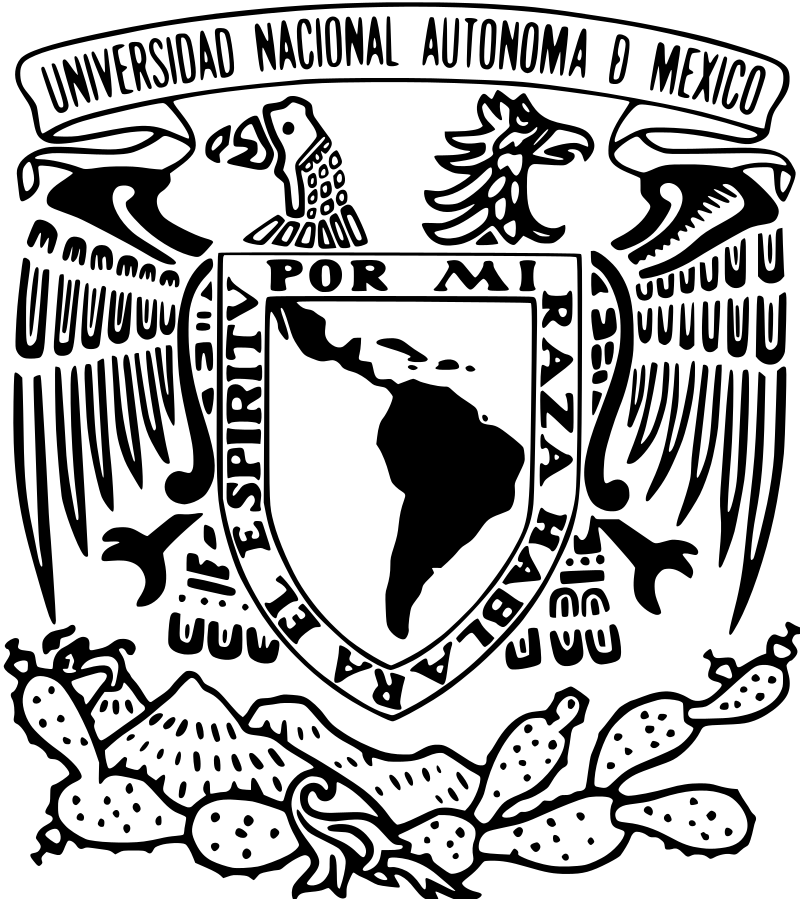
\includegraphics[width=4cm]{logo_unam.png}
  \label{EscudoUNAM}
  \endminipage
  \minipage{0.32\textwidth}
  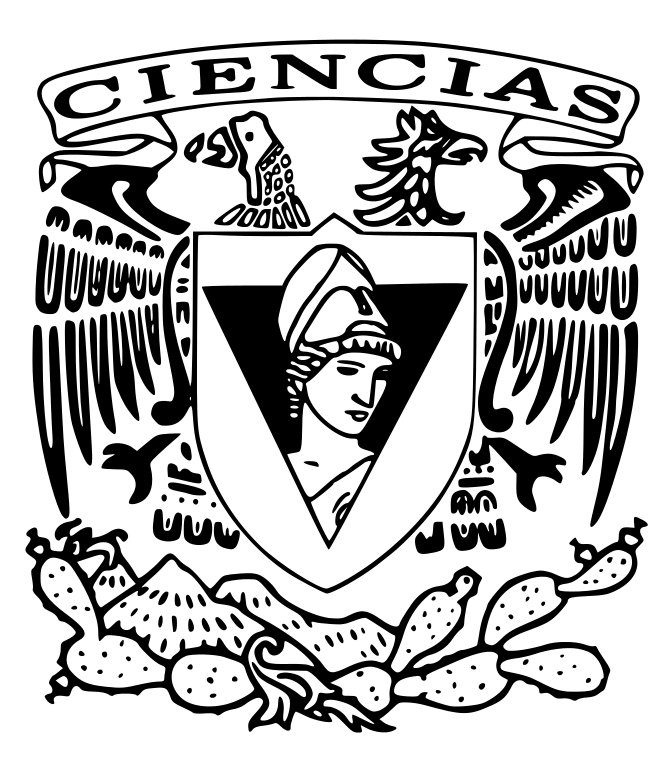
\includegraphics[height=4.9cm, width=4cm]{logo_ciencias.png}
  \label{EscudoFC}
  \endminipage
\end{figure}

\begin{center}
	\vspace{0.8cm}
	\LARGE
	UNIVERSIDAD NACIONAL AUTÓNOMA DE MÉXICO
  
	\vspace{0.8cm}
	\LARGE
  FACULTAD DE CIENCIAS
  
	\vspace{1.7cm}
	\Large
	\textbf{Reporte proyecto 2: Voyager (Administrador de audioteca digital).}
  
	\vspace{1.3cm}
	\normalsize
	PRESENTA \\
	\vspace{.3cm}
	\large
	\textbf{Bruno Bernardo Soto Lugo \\ 426008646}
  
	\vspace{1.3cm}
	\normalsize
	PROFESOR \\
	\vspace{.3cm}
	\large
	\textbf{Canek Peláez Valdés} \\

	\vspace{1.3cm}
	\normalsize
	AYUDANTES \\
	\vspace{.3cm}
	\large
	\textbf{Miriam Torres Bucio} \\
	\textbf{Cynthia Lizbeth Sánchez Urbano} \\
  
\end{center}

\newpage

\section{Introducción}
El presente documento detalla el proceso de desarrollo de \textbf{Voyager}, un sistema diseñado para la gestión y organización de audiotecas locales. El programa permite a los usuarios explorar, minar y visualizar colecciones de archivos de audio, extrayendo automáticamente metadatos como artistas, álbumes, géneros y carátulas de álbumes.

El sistema ha sido desarrollado utilizando el lenguaje \textbf{Kotlin} y el framework \textbf{Compose Multiplatform}. El desarrollo siguió el modelo de cascada, enfocándose en la definición clara de requisitos, el diseño de arquitectura robusta y la implementación técnica de los componentes de minería y persistencia.

\section{Análisis}
En esta fase se definieron las capacidades que el sistema debe ofrecer para garantizar una experiencia de usuario eficiente.

\subsection{Requisitos}
A partir de las especificaciones del programa, se identificaron los siguientes componentes clave:

\begin{itemize}
  \item \textbf{Minería de Archivos:} El sistema debe ser capaz de recorrer directorios de forma recursiva para localizar archivos compatibles. Debe identificar la ruta absoluta y los metadatos asociados.
  \item \textbf{Persistencia de Datos:} Los metadatos extraídos deben almacenarse en una base de datos.
  \item \textbf{Interfaz de Usuario (UI):} El sistema debe presentar una interfaz gráfica que permita navegar por álbumes, visualizar listas de canciones y mostrar detalles específicos de cada pista o artista.
  \item \textbf{Función de búsqueda} El sistema debe presentar una función de búsqueda que permita el uso de filtros.
\end{itemize}

%@startuml
%
%actor "Usuario" as User
%
%rectangle "Voyager - Sistema de Gestión de Audiotecas Locales" {
%
  %package "Interfaz de usuario" {
    %usecase "Importar audioteca" as UC_Import
    %usecase "Mostrar álbumes" as UC_Albums
    %usecase "Mostrar canciones" as UC_Songs
    %usecase "Mostrar detalles de pista" as UC_Track
    %usecase "Mostrar detalles de artista" as UC_Artist
    %usecase "Buscar con filtros" as UC_Search
  %}
%
  %package "Servicios internos" {
    %usecase "Recorrer directorios" as UC_Scan
    %usecase "Extraer metadatos" as UC_Metadata
    %usecase "Almacenar metadatos" as UC_Store
    %usecase "Obtener datos de la audioteca" as UC_Load
    %usecase "Ejecutar búsqueda" as UC_Query
  %}
%
  %UC_Import ..> UC_Scan : <<include>>
  %UC_Import ..> UC_Metadata : <<include>>
  %UC_Import ..> UC_Store : <<include>>
%
  %UC_Albums ..> UC_Load : <<include>>
  %UC_Songs ..> UC_Load : <<include>>
  %UC_Track ..> UC_Load : <<include>>
  %UC_Artist ..> UC_Load : <<include>>
%
  %UC_Search ..> UC_Query : <<include>>
  %UC_Query ..> UC_Load : <<include>>
%}
%
%User --> UC_Import
%User --> UC_Albums
%User --> UC_Songs
%User --> UC_Track
%User --> UC_Artist
%User --> UC_Search
%
%@enduml
\begin{figure}[H]
  \centering
  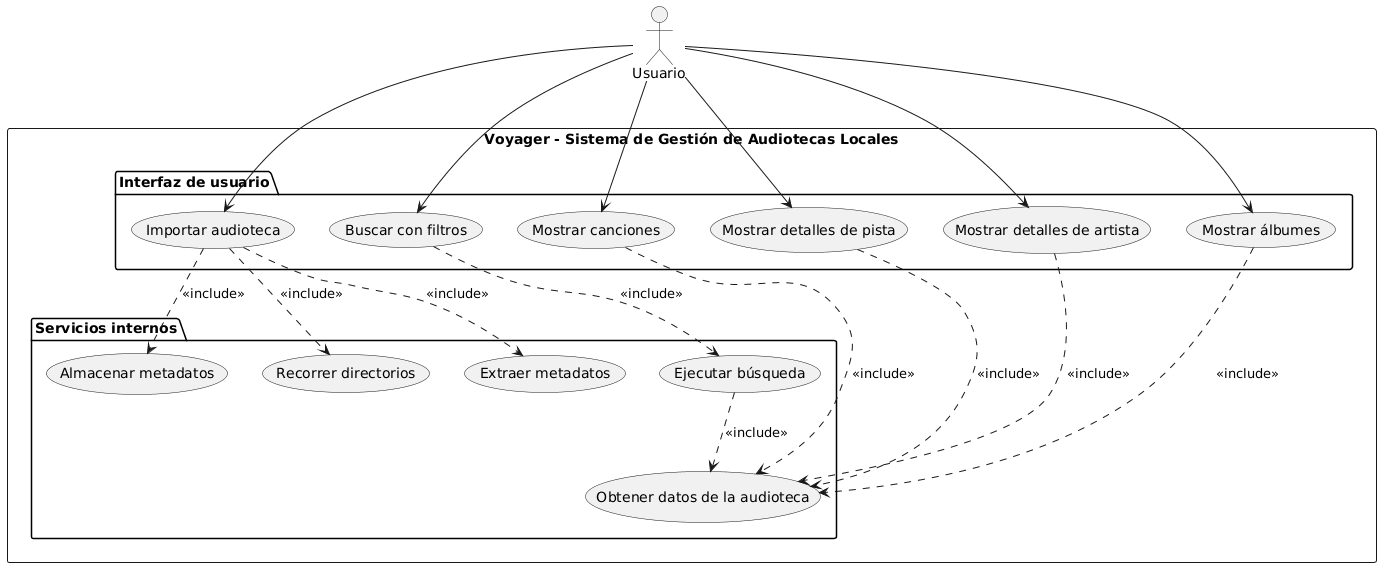
\includegraphics[width=13cm]{usecase.png}
  \caption{Diagrama de casos de uso de Voyager.}
\end{figure}

\section{Diseño}
El diseño de Voyager se centra en la separación de responsabilidades para facilitar la mantenibilidad del código. Para ello, el problema se divide en subproblemas y cada uno se asigna a un componente responsable.
 
\subsection{Descomposición en subproblemas}
\begin{table}[H]
  \centering
  \renewcommand{\arraystretch}{1.3}
  \begin{tabular}{|p{3.2cm}|p{7.2cm}|p{3.6cm}|}
    \hline
    \textbf{Subproblema} & \textbf{Responsabilidad} & \textbf{Componente} \\
    \hline
    Obtención de datos & Recorrer un directorio, localizar los archivos de audio y extraer sus metadatos y carátulas. & \texttt{Miner}, \texttt{SongMetadata} \\
    \hline
    Almacenamiento y consulta & Guardar los metadatos y responder las consultas de canciones, álbumes e intérpretes, incluida la búsqueda. & \texttt{DatabaseDriver}, entidades (\texttt{DbDataClasses}) \\
    \hline
    Presentación & Mostrar la audioteca, los detalles y los resultados, y capturar las acciones del usuario. & Pantalla principal y columnas \\
    \hline
    Coordinación & Recibir las acciones del usuario, iniciar la minería, almacenar lo encontrado y mantener el estado que la presentación necesita. & \texttt{MainController} \\
    \hline
  \end{tabular}
  \caption{Subproblemas de Voyager y el componente responsable de cada uno.}
  \label{tab:subproblemas}
\end{table}
 
\subsection{Patrón arquitectónico: MVC}
Los componentes se organizan según el patrón \textbf{MVC (Model-View-Controller)}, que separa los datos, su presentación y la lógica que coordina a ambos.
 
\begin{enumerate}
  \item \textbf{Model:} Agrupa los subproblemas de obtención de datos y de almacenamiento y consulta. El \texttt{DatabaseDriver} sigue el patrón DAO: concentra el acceso a los datos para que ningún otro componente conozca cómo se almacenan. El \texttt{Miner} no conoce ni el almacenamiento ni la interfaz: avisa de sus resultados mediante las notificaciones \texttt{onFound} (por cada canción encontrada) y \texttt{onFinish} (al terminar).
  \item \textbf{View:} Corresponde al subproblema de presentación. Está formada por la pantalla principal, las columnas (navegación, biblioteca de audio, carátulas de álbumes, información de canción y de álbum), los diálogos de edición y búsqueda y el reproductor de audio. Mantiene únicamente el estado visual (canción y álbum seleccionados, panel visible, reproductor activo), pide al usuario el directorio a minar y consulta al \texttt{DatabaseDriver} los datos que muestra.
  \item \textbf{Controller:} Corresponde al subproblema de coordinación. El \texttt{MainController} abre la base de datos al crearse, recibe de la vista el directorio elegido (\texttt{onDirectoryChosen}), crea e inicia el \texttt{Miner}, almacena cada canción encontrada con \texttt{saveSong} y libera los recursos en \texttt{close()}. Publica su estado (la base de datos disponible, si hay una minería en curso y la última canción encontrada) para que la vista lo observe.
\end{enumerate}
 
El usuario interactúa con la vista, la vista notifica al controlador, el controlador coordina al modelo y actualiza su estado, y la vista se actualiza y consulta al modelo para mostrar los datos.
 
\subsection{Decisiones de diseño}
\begin{itemize}
  \item \textbf{Desacoplamiento del Miner.} El \texttt{Miner} se comunica mediante notificaciones, de modo que puede reutilizarse sin depender del almacenamiento ni de la interfaz.
  \item \textbf{Minería asíncrona.} La minería se ejecuta de forma independiente de la interfaz para que esta no se bloquee. Como una nueva minería reemplaza a la anterior, el controlador debe ignorar los resultados de las mineras obsoletas.
  \item \textbf{Modelo de datos.} Las entidades son las canciones (rolas), los álbumes y los intérpretes. Los álbumes se identifican por el directorio que contiene a las canciones y no por la etiqueta de álbum.
  \item \textbf{Interfaz gráfica.} El diseño de la interfaz gráfica fue fuertemente inspirado por \textbf{Strawberry Music Player}, la preferencia personal para reproducción y administración de música.
\end{itemize}
 
\subsection{Diagramas UML}
\subsubsection{Diagrama de secuencia: proceso de minería}
 
%@startuml
%actor Usuario
%participant "View\n(Pantalla principal)" as V
%participant "Controller\n(MainController)" as C
%box "Model"
  %participant "Miner" as Miner
  %participant "DatabaseDriver" as DB
%end box
%database "Disco" as Disco
%
%Usuario -> V : Pulsa botón de añadir
%V -> Usuario : Solicita un directorio
%Usuario --> V : Elige un directorio
%V -> C : onDirectoryChosen(path)
%C -> Miner : Crea el Miner con onFound y onFinish
%C -> Miner : Inicia la minería recursiva
%loop por cada archivo de audio
  %Miner -> Disco : Lee etiquetas y portada
  %Disco --> Miner : Etiquetas y portada
  %Miner -> Disco : Guarda la portada
  %Miner -> C : onFound(SongMetadata)
  %C -> DB : saveSong(metadata)
  %C -> C : Actualiza su estado
  %C --> V : El estado cambia
  %V -> DB : Consulta canciones y álbumes
  %DB --> V : Rolas y álbumes
  %V --> Usuario : Muestra la canción
%end
%Miner -> C : onFinish()
%C -> C : Marca la minería como terminada
%@enduml
 
\begin{figure}[H]
  \centering
  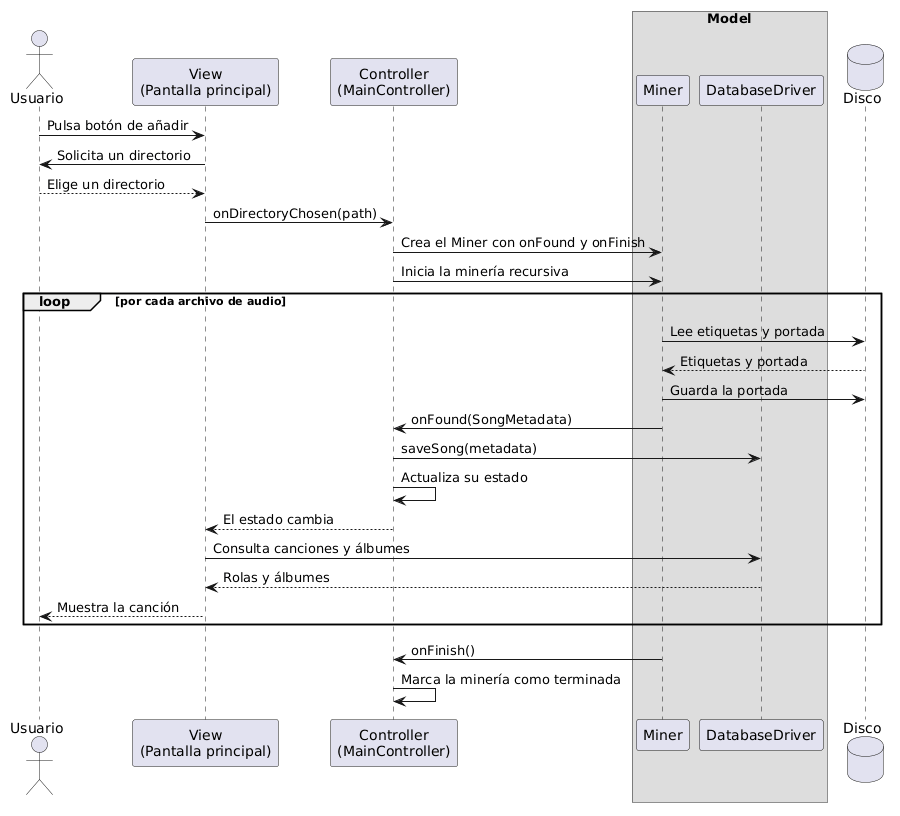
\includegraphics[width=13cm]{minerdiagram.png}
  \caption{Diagrama de secuencia del proceso de minería de archivos.}
\end{figure}
 
\subsubsection{Diagrama de arquitectura MVC}
 
%@startuml
%package "View" {
  %[Pantalla principal y columnas] as V
  %[Reproductor de audio] as Player
%}
%package "Controller" {
  %[MainController] as C
%}
%package "Model" {
  %[Miner] as Miner
  %[SongMetadata] as Meta
  %[DatabaseDriver] as DB
  %[Entidades] as Data
%}
%V --> C : Acciones del usuario
%V --> Player : Reproducción
%V --> DB : Consultas de lectura
%C --> Miner : Crea e inicia
%Miner ..> C : onFound, onFinish
%C --> DB : Almacena canciones
%Miner ..> Meta : Produce
%DB ..> Data : Usa entidades
%@enduml
 
\begin{figure}[H]
  \centering
  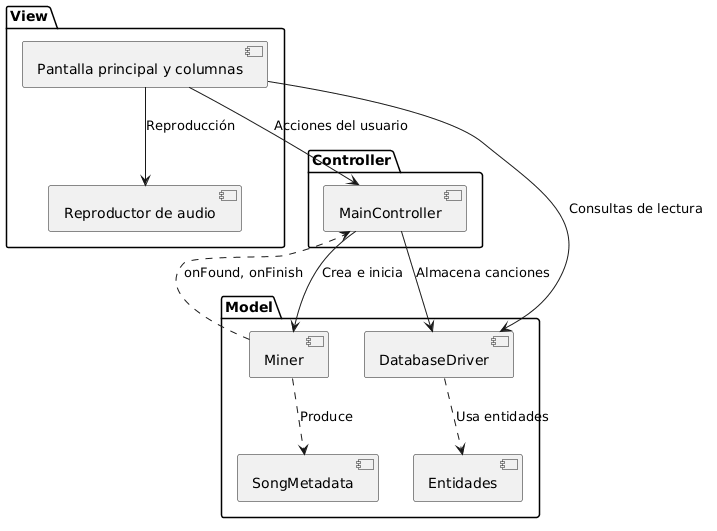
\includegraphics[width=0.8\textwidth]{mvc.png}
  \caption{Diagrama de arquitectura MVC del sistema Voyager.}
\end{figure}
 
\section{Desarrollo}
El desarrollo consistió en elegir las tecnologías con las que se realizó cada componente del diseño.
 
\subsection{Tecnologías generales}
Se seleccionó \textbf{Kotlin} por su sintaxis concisa, su similitud a Java, su paradigma orientado a objetos, su manejo de funciones fuera de clases y por características como las corrutinas, que permiten manejar operaciones de entrada y salida pesadas de manera asíncrona. La interfaz se construyó con \textbf{Compose Multiplatform} y \textbf{Material 3}, que permiten crear una interfaz reactiva.
 
\subsection{Obtención de datos: Miner}
El recorrido recursivo del directorio se implementó con \texttt{File.walkTopDown()}, filtrando los archivos \texttt{.mp3} y \texttt{.flac}. Las etiquetas (título, artista, álbum, pista, año y género) se leen con la biblioteca \textbf{JAudioTagger}. Las carátulas se extraen del archivo, se convierten a JPEG con \texttt{javax.imageio.ImageIO} y se guardan en un directorio de caché.
 
Para evitar que la interfaz se congele durante el escaneo del disco se utilizó un \textbf{CoroutineScope} con \texttt{Dispatchers.IO}. Las notificaciones \texttt{onFound} y \texttt{onFinish} del diseño se implementaron como funciones de Kotlin recibidas por el constructor de la clase.
 
\subsection{Almacenamiento y consulta: DatabaseDriver}
Se utilizó \textbf{SQLite} mediante \textbf{JDBC}. La base de datos es un archivo (\texttt{songlibrary.db}) en el directorio \texttt{\textasciitilde/.local/share/voyager/}, cuyo esquema se crea la primera vez que se ejecuta el programa. Las clases de datos en \texttt{DbDataClasses.kt} incluyen métodos \texttt{fromSqlResult} para mapear directamente los registros de la base de datos a objetos de Kotlin.
 
\subsection{Presentación: interfaz de usuario}
Cada columna de la vista es una función composable de Compose Multiplatform. El estado visual (canción y álbum seleccionados, panel visible y reproductor activo) se conserva con \texttt{remember} y \texttt{mutableStateOf}. El selector de directorios utiliza \texttt{JFileChooser} de Swing, y la reproducción de audio se realiza con la biblioteca \textbf{Gadulka}.
 
\subsection{Coordinación: MainController}
El \texttt{MainController} es una clase de Kotlin independiente de los composables, que solo utiliza \texttt{mutableStateOf} (del runtime de Compose) para publicar su estado: la base de datos disponible, si hay una minería en curso y la última canción encontrada, de modo que Compose actualiza la interfaz cuando cambian. Como las notificaciones del \texttt{Miner} se ejecutan en un hilo distinto al de la interfaz, cada minería recibe un número de ejecución (\texttt{runNumber}) y los resultados de las ejecuciones obsoletas se descartan.
 
\section{Conclusiones}
La implementación del proyecto Voyager permitió consolidar conocimientos en arquitectura de software, bases de datos relacionales, programación concurrente y manejo de sistemas de archivos. El uso del modelo de cascada facilitó una comprensión clara de los requerimientos antes de iniciar el código, lo que redujo la necesidad de refactorizaciones estructurales, aunque inevitablemente se tuvieron que modificar varias partes del modelo ya definidas por no pensar en alguna limitación o por la existencia de errores clave.
 
El uso del patrón MVC permitió que la lógica de minería y de acceso a los datos sea independiente de la representación visual, y que el controlador concentre la coordinación entre ambas.

La mayor limitación del proyecto fue la falta de creación de pruebas unitarias. Con ellas, el desarrollo hubiera sido acelerado. Las pruebas de correcto funcionamiento se realizaron utilizando la interfaz gráfica misma y verificando la inserción adecuada dentro de la base de datos utilizando el programa \textbf{DBeaver}.
 
Como trabajo futuro se sugiere:
\begin{itemize}
  \item Lograr que el método \texttt{stop()} del \texttt{Miner} interrumpa realmente el recorrido en curso; actualmente los resultados de una minería detenida solo se descartan en el controlador.
  \item Hacer que todas las consultas de la vista pasen por el controlador, en lugar de que las columnas accedan directamente al \texttt{DatabaseDriver}.
  \item Implementar pruebas unitarias para garantizar el adecuado desarrollo del programa.
\end{itemize}

\end{document}
